\documentclass[conference]{IEEEtran}
\IEEEoverridecommandlockouts
\usepackage[utf8]{inputenc}
\usepackage[T1]{fontenc}
\usepackage{cite}
\usepackage{amsmath,amssymb,amsfonts}
\usepackage{algorithmic}
\usepackage{graphicx}
\usepackage{textcomp}
\usepackage{xcolor}
\usepackage{booktabs}
\usepackage{multirow}
\usepackage{listings}
\usepackage{url}
\usepackage{tikz}
\usepackage{pgfplots}
\pgfplotsset{compat=1.16}
\usetikzlibrary{shapes.geometric, arrows.meta, positioning, calc}

\newtheorem{proposition}{Proposition}

\lstset{
    basicstyle=\ttfamily\scriptsize,
    breaklines=true,
    frame=single,
    numbers=left,
    numberstyle=\tiny,
    keywordstyle=\color{blue}\bfseries,
    commentstyle=\color{gray}\itshape,
    stringstyle=\color{red!70!black}
}

\def\BibTeX{{\rm B\kern-.05em{\sc i\kern-.025em b}\kern-.08em
    T\kern-.1667em\lower.7ex\hbox{E}\kern-.125emX}}

\begin{document}

\title{Hardware-Agnostic Lexical AEAD Codebook Concealment via Pure-Python ChaCha20-Poly1305: Canonical Framing, Avalanche Dynamics, and Heuristic DPI Evasion}

\author{\IEEEauthorblockN{Carlos Andr\'e Sousa}
\IEEEauthorblockA{\textit{Master in Cybersecurity and Computer Systems Auditing} \\
\textit{ISPGAYA, Instituto Superior Polit\'ecnico Gaya} \\
Vila Nova de Gaia, Portugal \\
Email: casousa@ispgaya.pt}
}

\maketitle

\begin{abstract}
Monitored communication channels expose a tension between confidentiality and traffic stealth: standard symmetric encryption produces high-entropy binary payloads that trigger stateless Deep Packet Inspection (DPI) heuristics, non-printable byte filters, and automated perimeter firewalls. Historical nomenclators and codebooks avoided binary framing by substituting operational terms with ordinary words, yet suffered from monoalphabetic frequency leakage, ciphertext malleability, and catastrophic key or dictionary compromise. This paper designs, formally analyzes, implements, and evaluates a pure-Python Lexical Authenticated Encryption with Associated Data (AEAD) engine requiring zero third-party libraries. Built atop RFC 8439 ChaCha20-Poly1305, the architecture decouples an operational command vocabulary from a benign cover lexicon of dimension $N$, maps tokens over the modular ring $\mathbb{Z}_N$, derives per-token shifts from ChaCha20 keystreams with exact rejection sampling, serializes the 96-bit CSPRNG nonce and 128-bit Poly1305 tag into canonical base-$N$ cover tokens, and supports authenticated randomized bucket padding. We prove a Base-$N$ Divisibility Proposition showing that non-power-of-two vocabularies such as $N=20$ induce non-canonical encoding malleability (mitigated via strict range checks) and deterministic most-significant-token distinguishers (observed empirically: only $2/20$ nonce-MSB words and $7/20$ tag-MSB words appear, $p < 10^{-100}$), whereas byte-aligned $N=256$ eliminates modulo bias, non-canonical encodings, and MSB leakage simultaneously ($256/256$ coverage, $p \ge 0.943$). The engine achieves 100\% bit-for-bit parity across all bytes of IETF RFC 8439 Sections 2.3.2 (64 bytes), 2.5.2, and 2.8.2 (114-byte ciphertext and 16-byte tag), satisfies Strict Avalanche Criterion targets ($49.91\%$ key diffusion, $t=-0.668, p=0.505$; $49.97\%$ nonce diffusion, $t=-0.258, p=0.797$), and masks an 85\%-skewed plaintext ($H=4.3202$ bits/symbol, $\chi^2=11.8, p=0.895, r_1=+0.0053$). In simulated stateless perimeter DPI trials across 10,000 packets covering short (6-word) and extended (60-word) regimes, our decoupled $\mathbb{Z}_{256}$ Lexical AEAD achieves 100\% evasion across byte-entropy ($H_b = 3.8660$ vs. $7.5673$ for raw RFC 8439), printability, and keyword-watchlist filters, while reducing wire footprint by 82.0\% ($587.4$~B vs. $3,256.2$~B) and accelerating throughput by $4.7\times$ ($444.9$~k vs. $94.2$~k tokens/s) compared to standard RFC 8439 paired with Base-256 word encoding. Across 1,000 tampering trials spanning ciphertext, nonce preamble, tag suffix, AAD, out-of-vocabulary, and non-canonical overflow attacks, authentication rejected 100.0\% of forged frames. A red-team likelihood-ratio detector separates our uniform cover-word stream from Zipf prose with 99\% to 100\% accuracy, which delimits the scheme to stateless perimeter filters.
\end{abstract}

\begin{IEEEkeywords}
Authenticated Encryption, ARX Ciphers, ChaCha20-Poly1305, Deep Packet Inspection Evasion, Information Theory, Lexical Steganography, Pure-Python Implementation, Strict Avalanche Criterion.
\end{IEEEkeywords}

\section{Introduction and Problem Formulation}
\label{sec:intro}

Modern symmetric encryption primitives prioritize provable indistinguishability and software throughput. Standardized AEAD constructions such as AES-GCM and ChaCha20-Poly1305 transform structured plaintexts into binary bitstrings statistically indistinguishable from uniform random noise \cite{rfc8439, gentile2024overlay, anyam2025empirical}.

In censored, audited, or adversarial network environments, uniform binary output creates a secondary operational exposure. Payloads exhibiting high byte entropy (approaching $8.0$ bits/byte on extended frames), low printable ASCII ratios, and rigid tunnel headers are flagged immediately by Deep Packet Inspection (DPI) middleboxes, stateful perimeter firewalls, and machine-learning flow classifiers \cite{mohd2026covertchannel, sun2022deep, alazzam2026advanced}. Even when the underlying cipher resists cryptanalysis, detection of an unauthorized encrypted channel triggers throttling, packet dropping, or endpoint isolation.

Overlay VPN benchmarks confirm that ChaCha20-Poly1305 excels on general-purpose processors lacking hardware cryptographic extensions such as AES-NI or ARMv8 Crypto \cite{anyam2025empirical, nianc2022symmetric}. Standard tunnel protocols nevertheless emit raw binary envelopes whose structural and statistical profiles are readily isolated by network telemetry pipelines and high-speed DPI schedulers \cite{jiang2021a, gentile2024overlay}.

Classical nomenclators and substitution codebooks attempted to conceal traffic structure by replacing operational terms with ordinary lexicon entries \cite{shannon1949communication, serret2022linguistic}. Although such payloads bypass binary-format filters, static codebooks fail catastrophically against basic cryptanalysis:
\begin{enumerate}
    \item \textbf{Monoalphabetic Frequency Leakage:} Deterministic word-to-word mappings preserve plaintext term distributions, exposing operational intent to frequency analysis and known-plaintext recovery \cite{shannon1949communication}.
    \item \textbf{Absence of Per-Message State:} Static dictionaries lack nonce diversification, collapsing across all past and future sessions if the table leaks.
    \item \textbf{Ciphertext Malleability:} Unauthenticated modular substitutions allow active Man-in-the-Middle adversaries to modify words without detection.
    \item \textbf{Periodic and Structural Weakness:} Short-period polyalphabetic ciphers such as Vigen\`ere collapse under index-of-coincidence analysis and autocorrelation tests, motivating modern pseudorandom stream generators resistant to linear and differential-linear attacks \cite{canteaut2025linear, todo2024differentiallinear}.
\end{enumerate}

A natural engineering baseline is to apply standard binary RFC 8439 ChaCha20-Poly1305 to UTF-8 text and map every output byte onto a 256-word benign dictionary (analogous to PGP Word List or BIP-39 encoding). While cryptographically sound, byte-level lexical encoding expands each 7-byte plaintext word into roughly 7 cover words, inflating a 60-word operational report to over $3.2$~KB and exceeding the 1,500-byte Ethernet MTU.

To overcome both classical codebook insecurity and naive byte-to-word expansion, this paper presents a hardware-agnostic, zero-third-party-dependency Lexical AEAD engine written in pure Python 3. The design couples RFC 8439 ChaCha20-Poly1305 \cite{rfc8439, bernstein2008chacha} with direct modular encryption over $\mathbb{Z}_N$ and decouples the operational vocabulary $\mathcal{V}_{\text{op}}$ from an everyday benign cover lexicon $\mathcal{V}_{\text{cover}}$. Each operational word maps to a single cover token rather than multiple encoded UTF-8 bytes, while the 96-bit CSPRNG nonce and 128-bit Poly1305 tag serialize canonically into cover tokens.

Our specific contributions are fivefold:
\begin{enumerate}
    \item \textbf{Pure-Python Decoupled Lexical AEAD Engine:} A dependency-free implementation of RFC 8439 ChaCha20-Poly1305 over $\mathbb{Z}_N$ featuring a 256-word benign cover lexicon decoupled from sensitive operational commands, CSPRNG nonce generation (\texttt{os.urandom}), Authenticated Associated Data (AAD), strict canonical range validation, constant-time tag comparison, and authenticated randomized bucket padding. Every byte of RFC 8439 Sections 2.3.2 (64 bytes), 2.5.2, and 2.8.2 (114-byte ciphertext plus 16-byte tag) is verified bit-for-bit.
    \item \textbf{Base-$N$ Divisibility Analysis and Anti-Malleability Proof:} We formalize the divisibility condition governing base-$N$ framing and prove empirically that non-power-of-two lexicons ($N=20$) suffer from non-canonical encoding malleability (eliminated via upper-bound checks) and severe MSB-token distinguishers ($2/20$ nonce-MSB and $7/20$ tag-MSB coverage), whereas $N=256$ eliminates all three artifacts simultaneously.
    \item \textbf{Cryptanalytic Benchmarking with Native Hypothesis Testing:} Multi-trial empirical evaluation ($R=30$ repetitions) covering SAC diffusion, Shannon entropy, Chi-Square uniformity with exact pure-Python $p$-values, lag-1 serial autocorrelation, rejection sampling ($\Delta p = 0$), and lexicon scalability ($N \in \{16, 20, 64, 128, 256\}$).
    \item \textbf{Head-to-Head Baseline Comparison:} Direct wire-footprint, latency, and throughput comparison against Standard RFC 8439 paired with Base-256 cover encoding, demonstrating up to 82.0\% bandwidth reduction and $4.7\times$ higher token throughput.
    \item \textbf{Two-Regime Simulated Heuristic DPI and Multi-Vector Tamper Evaluation:} Stateless perimeter DPI experiments across 10,000 packets spanning short (6-word) and extended (60-word) payloads, decomposing byte-entropy, printability, and keyword-watchlist alerts alongside 1,000 four-vector tampering trials (100.0\% rejection).
\end{enumerate}

\section{State of the Art and Related Literature}
\label{sec:state_of_art}

\subsection{Traffic Fingerprinting and Perimeter Inspection}
Network defense systems detect covert or encrypted flows through structural and statistical telemetry without breaking the underlying cipher. Converting packet sequences into block-image representations allows convolutional neural classifiers to separate VPN tunnels with high precision \cite{sun2022deep}. Transformer-based website fingerprinting extends this capability by exploiting burst timing and packet-size distributions across censored VPN links \cite{alazzam2026advanced}. Production overlay deployments such as WireGuard and OpenVPN exhibit distinct flow entropy and binary framing profiles visible to passive monitors \cite{gentile2024overlay, anyam2025empirical}. Bit-level randomness heuristics flag encrypted covert payloads at perimeter gateways \cite{mohd2026covertchannel}, including clustered line-rate DPI appliances scheduled via P4 pipelines \cite{jiang2021a}. Under stringent traffic policing, short-packet covert schemes rely on channel truncation and format reshaping to lower detection probability \cite{lu2023channel}.

\subsection{Linguistic Steganography and Format-Preserving Encryption}
Classical secrecy theory establishes that perfect secrecy demands key entropy at least matching message entropy \cite{shannon1949communication}. Linguistic steganography embeds ciphertext within natural-language tokens for messaging channels \cite{serret2022linguistic}. Reversible frameworks leverage Bayesian masked language models to preserve grammatical coherence during embedding \cite{chang2023reversible}, while foundation-model approaches such as StegGPT and StegoZip combine large language models with character-level embedding or compression to improve payload capacity \cite{adeeb2025steggpt, jiang2025stegozip}. Nevertheless, multi-granularity neural steganalysis reliably identifies synthetic LLM-generated text distributions \cite{wang2025multiclassification}, showing that generative prose incurs substantial computational cost while remaining vulnerable to dedicated linguistic detectors.

In contrast, Format-Preserving Encryption (FPE) enforces exact output domain membership without heavy neural inference. Multilayer textual schemes combine FPE with Huffman coding for structured concealment \cite{majeed2022new}, though Feistel-based FPE over small domains requires careful round bounds to prevent small-domain cryptanalytic attacks \cite{roh2026security}. Pure-Python cryptographic prototypes have likewise demonstrated practical linguistic encryption for non-Latin scripts without native binary extensions \cite{prabu2023implementation}.

\subsection{ARX Stream Ciphers and Platform Independence}
Ciphers built on Addition, Rotation, and XOR (ARX) primitives execute efficiently on commodity arithmetic logic units without hardware cryptographic coprocessors \cite{bernstein2008chacha, rfc8439}. Table-lookup AES implementations face cache-timing side channels on CPUs and GPUs when hardware AES-NI instructions are unavailable \cite{ahn2021trident}, motivating S-Box hardening studies \cite{topanto2022security} and S-Box-free ARX alternatives.

Recent hardware and software studies confirm ARX versatility across deployment tiers. Sparse parallel prefix adders accelerate pipelined ChaCha20 silicon cores \cite{rashidi2025highperformance}, while modified quarter-round proposals investigate algebraic diffusion trade-offs \cite{kebande2023extendedchacha}. On constrained edge devices, in-memory ChaCha20 architectures suppress physical side-channel leakage \cite{aamir2021chacha20}, and hybrid ECC-ChaCha20 constructions secure medical IoT telemetry \cite{sethi2025lightweight}. Empirical RISC-V evaluations further show that ARX stream ciphers outperform unaccelerated block ciphers in cycles per byte \cite{nianc2022symmetric}, complementing standardized lightweight AEAD permutations such as Ascon \cite{dobraunig2021ascon}.

\subsection{Cryptanalytic Bounds on Stream and Symmetric Primitives}
Symmetric stream security is benchmarked against linear, differential-linear, and rotational cryptanalysis \cite{canteaut2025linear, biryukov2025linear, todo2024differentiallinear}. For reduced-round ChaCha variants, refined linear approximations and revamped differential-linear distinguishers have pushed key-recovery and distinguishing trails up to 7 rounds \cite{coutinho2021improved, dey2022revamped, beierle2022improved}, complemented by rotational and higher-order differential-linear analyses \cite{barbero2022rotational, ghafoori2024higherorder}. Parallel automated differential-linear search methods continue to advance cryptanalysis across lightweight symmetric families such as SIMON-like ciphers and GIFT \cite{lv2026automated, wang2024differentiallinear}, yet full 20-round ChaCha20 maintains a substantial security margin against all known attacks.

Empirical diffusion and keystream uniformity distinguish robust designs from legacy or flawed generators. Legacy RC4 variants suffer from measurable avalanche and state-bias weaknesses \cite{madarrocap2021measuring}, while standardized stream ciphers such as ZUC undergo intensive design and cryptanalytic scrutiny to rule out linear and initialization biases \cite{mukherjee2021design, mukherjee2021cryptanalysis}. Unconventional heuristic models such as DNA-splicing cryptanalysis have also been explored against unknown stream generators \cite{yaseen2021splicing}. Strict Avalanche Criterion (SAC) testing remains a standard diagnostic across ARX-based sub-functions, as demonstrated recently on SHA-256 component combinations \cite{vaughn2026relaxation}.

\subsection{Positioning Against Related Approaches}
Table~\ref{tab:related} positions our design against the approaches discussed above along five operational axes. Entries for related work are qualitative readings of the cited descriptions (n/e: not evaluated in this work); entries for the schemes we implemented are backed by the measurements of Section~\ref{sec:eval}.

\begin{table*}[t]
\caption{Qualitative Positioning of Lexical AEAD Against Related Concealment Approaches}
\label{tab:related}
\centering
\resizebox{\textwidth}{!}{%
\begin{tabular}{lccccc}
\toprule
\textbf{Approach} & \textbf{Native AEAD} & \textbf{F1/F2 stealth} & \textbf{F3 keyword stealth} & \textbf{Single-MTU @ 60 words} & \textbf{Zipf / $n$-gram stealth} \\
\midrule
Static codebook / nomenclator \cite{shannon1949communication} & No & Yes & No & Yes & Partial \\
Raw RFC 8439 binary \cite{rfc8439} & Yes & No & Yes & Yes & No \\
Feistel FPE over small domain \cite{roh2026security, majeed2022new} & No & Yes & n/e & Yes & No \\
LLM linguistic steganography \cite{adeeb2025steggpt, jiang2025stegozip} & No & Yes & Yes & n/e & Partial \cite{wang2025multiclassification} \\
RFC 8439 + Base-256 words (baseline) & Yes & Yes & Yes & No ($3{,}256$~B) & No \\
\textbf{Lexical AEAD $\mathbb{Z}_{256}$ (ours)} & \textbf{Yes} & \textbf{Yes} & \textbf{Yes} & \textbf{Yes} ($587$~B) & \textbf{No} (Sec.~\ref{sec:redteam}) \\
\bottomrule
\end{tabular}%
}
\end{table*}

\section{Cryptographic Architecture and Formal Analysis}
\label{sec:arch}

\subsection{RFC 8439 ChaCha20 State and ARX Rounds}
ChaCha20 maintains a 512-bit internal state matrix $\mathbf{S}$ structured as sixteen 32-bit unsigned words:
\begin{equation}
\mathbf{S}_0 = \begin{pmatrix} 
c_0 & c_1 & c_2 & c_3 \\ 
k_0 & k_1 & k_2 & k_3 \\ 
k_4 & k_5 & k_6 & k_7 \\ 
b_0 & n_0 & n_1 & n_2 
\end{pmatrix}
\end{equation}
where $c_0, \dots, c_3$ encode the ASCII constant \texttt{"expand 32-byte k"} in little-endian order ($0\text{x}61707865$, $0\text{x}3320646\text{e}$, $0\text{x}79622\text{d}32$, $0\text{x}6\text{b}206574$), $k_0, \dots, k_7$ store the 256-bit secret key, $b_0 \in [0, 2^{32}-1]$ is the 32-bit block counter, and $n_0, n_1, n_2$ encode the 96-bit nonce \cite{rfc8439, rashidi2025highperformance}.

Each Quarter-Round $\text{QR}(a, b, c, d)$ applies modular 32-bit addition ($\boxplus$), bitwise XOR ($\oplus$), and circular left rotation ($\lll$):
\begin{align}
a &\leftarrow (a \boxplus b) \pmod{2^{32}}, & d &\leftarrow (d \oplus a) \lll 16 \\
c &\leftarrow (c \boxplus d) \pmod{2^{32}}, & b &\leftarrow (b \oplus c) \lll 12 \\
a &\leftarrow (a \boxplus b) \pmod{2^{32}}, & d &\leftarrow (d \oplus a) \lll 8 \\
c &\leftarrow (c \boxplus d) \pmod{2^{32}}, & b &\leftarrow (b \oplus c) \lll 7
\end{align}

Ten double-rounds (20 rounds total, alternating 4 column and 4 diagonal quarter-rounds) produce $\mathbf{S}_{20}$. The 64-byte keystream block $\mathbf{Z}$ adds the initial state back word-wise in little-endian serialization:
\begin{equation}
\mathbf{Z} = (\mathbf{S}_{20} \boxplus \mathbf{S}_0) \pmod{2^{32}}
\end{equation}

\subsection{Decoupled Cover Lexicon Mapping over Ring $\mathbb{Z}_N$}
Prior lexical prototypes that encrypt operational terms back into the same tactical wordlist expose sensitive keywords (such as \texttt{atacar} or \texttt{evacuar}) directly on the wire, triggering trivial IDS watchlist rules. To eliminate semantic keyword leakage, our architecture decouples two vocabularies:
\begin{itemize}
    \item An \textbf{operational plaintext lexicon} $\mathcal{V}_{\text{op}}$ of size $M \le N$ with injective index map $\psi: \mathcal{V}_{\text{op}} \hookrightarrow \mathbb{Z}_N$ (in our tactical scenario, $M=20$ commands).
    \item A \textbf{benign cover lexicon} $\mathcal{V}_{\text{cover}} = \{w_0, \dots, w_{N-1}\}$ disjoint from $\mathcal{V}_{\text{op}}$ ($\mathcal{V}_{\text{op}} \cap \mathcal{V}_{\text{cover}} = \emptyset$), with bijection $\phi: \mathcal{V}_{\text{cover}} \to \mathbb{Z}_N$. Our optimal profile instantiates $N=256$ everyday lowercase ASCII words (objects, nature, daily logistics).
\end{itemize}

For a plaintext sequence $P = (p_0, \dots, p_{m-1}) \in \mathcal{V}_{\text{op}}^m$, the engine extracts one byte $K_i = z_i$ per token (64 tokens per ChaCha20 block, no keystream wasted) when $N \mid 256$, and otherwise 16-bit unsigned integers $K_i = (z_{2i} \ll 8) \mid z_{2i+1}$, from ChaCha20 blocks starting at counter $b_0 \ge 1$. When $2^{16} \not\equiv 0 \pmod N$, exact rejection sampling discards samples $K_i \ge L = 65,536 - (65,536 \bmod N)$ before computing $D_i = K_i \bmod N$, guaranteeing $\Pr[D_i = r] = 1/N$ ($\Delta p = 0.00$). When $N = 2^b$ with $b \le 16$ (such as $N=256$), $L = 65,536$, requiring zero rejections and strictly deterministic execution. Encryption and decryption operate over $\mathbb{Z}_N$:
\begin{align}
C_i &= \phi^{-1}\left( (\psi(p_i) + D_i) \pmod N \right) \in \mathcal{V}_{\text{cover}} \\
p_i &= \psi^{-1}\left( (\phi(C_i) - D_i) \pmod N \right) \in \mathcal{V}_{\text{op}}
\end{align}
Repeated plaintext tokens map to independent cover words ($p_i = p_j \nRightarrow C_i = C_j$ for $i \neq j$), and zero operational keywords ever appear on the wire.

\subsection{Canonical Base-$N$ AEAD Framing and Divisibility Condition}
To eliminate binary headers and authentication tags on monitored channels, the 96-bit CSPRNG nonce $V \in [0, 2^{96}-1]$ and 128-bit Poly1305 tag $T \in [0, 2^{128}-1]$ are serialized into $k = \lceil 96 / \log_2 N \rceil$ preamble tokens and $t = \lceil 128 / \log_2 N \rceil$ suffix tokens from $\mathcal{V}_{\text{cover}}$:
\begin{equation}
V = \sum_{j=0}^{k-1} d_j N^j, \qquad T = \sum_{j=0}^{t-1} g_j N^j, \qquad d_j, g_j \in \mathbb{Z}_N
\end{equation}

Following RFC 8439 Sections 2.6 and 2.8, block counter $b_0 = 0$ derives the 32-byte one-time Poly1305 key $(r, s)$ with clamped $r$. Let $\mathcal{C}_{\text{utf8}}$ denote the canonical space-delimited ASCII/UTF-8 serialization of $(C_0, \dots, C_{m-1})$. The Poly1305 MAC evaluates over prime $2^{130}-5$ on:
\begin{equation}
\mathcal{M} = \text{AAD} \mathbin{\Vert} \mathbf{0}_{p_1} \mathbin{\Vert} \mathcal{C}_{\text{utf8}} \mathbin{\Vert} \mathbf{0}_{p_2} \mathbin{\Vert} [\text{len}(\text{AAD})]_8 \mathbin{\Vert} [\text{len}(\mathcal{C}_{\text{utf8}})]_8
\end{equation}
producing wire packet $\text{Pkt} = \text{Preamble}_k \mathbin{\Vert} C_0 \cdots C_{m-1} \mathbin{\Vert} \text{Tag}_t \in \mathcal{V}_{\text{cover}}^{k+m+t}$.

A critical subtlety arises when $N$ is not an exact power of two. For $N=20$, $k=23$ and $t=30$, yielding $20^{23} \approx 10.58 \cdot 2^{96}$ and $20^{30} \approx 3.15 \cdot 2^{128}$. This creates two cryptographic hazards:
\begin{enumerate}
    \item \textbf{Non-Canonical Encoding Malleability:} A naive base-$N$ decoder that truncates reconstructed integers to 96 or 128 bits accepts forged encodings $V' = V + c \cdot 2^{96}$ or $T' = T + c \cdot 2^{128}$ ($c \ge 1$). An active adversary can alter all 23 nonce tokens or all 30 tag tokens and still pass Poly1305 verification. Our engine eliminates this attack for arbitrary $N$ by strictly rejecting any decoded integer satisfying $V \ge 2^{96}$ or $T \ge 2^{128}$ prior to decryption.
    \item \textbf{Most-Significant-Token Distinguisher:} Even with canonical bounds enforced, valid integers $V < 2^{96}$ force the top base-20 digit $d_{22} = \lfloor V / 20^{22} \rfloor \in \{0, 1\}$, meaning token \#23 of every packet can take only 2 of 20 words. Likewise, $g_{29} = \lfloor T / 20^{29} \rfloor \in \{0, \dots, 6\}$ restricts the final packet token to 7 of 20 words, creating a trivial deterministic fingerprint.
\end{enumerate}

\begin{proposition}[Base-$N$ Divisibility Condition]
For 96-bit nonces, 128-bit tags, and 16-bit keystream sampling, a Lexical AEAD packet achieves simultaneous zero modulo truncation bias ($\Delta p = 0$ without rejection sampling), zero non-canonical wire encodings ($N^k = 2^{96}$ and $N^t = 2^{128}$), and strictly uniform MSB-token distributions across $\mathcal{V}_{\text{cover}}$ if and only if $N = 2^b$ where $b \mid \gcd(96, 128, 16) = 16$, i.e., $N \in \{2, 4, 16, 256, 65536\}$.
\end{proposition}

\textit{Proof Sketch:} Zero modulo bias on 16-bit integers requires $N \mid 2^{16}$, hence $N = 2^b$ with $b \in \{1, \dots, 16\}$. Exact bijectivity and zero MSB truncation on 96-bit nonces and 128-bit tags require $N^k = 2^{bk} = 2^{96}$ and $N^t = 2^{bt} = 2^{128}$, equivalently $b \mid 96$ and $b \mid 128$. Combining all three constraints yields $b \mid \gcd(96, 128, 16) = 16$, so $b \in \{1, 2, 4, 8, 16\}$. $\square$

Choosing $N = 256$ ($b = 8$) satisfies Proposition~1 with minimal practical vocabulary size, fixing $k = 12$ nonce tokens and $t = 16$ tag tokens ($28$ total metadata tokens, down from $53$ at $N=20$).

\begin{figure}[htbp]
\centering
\resizebox{\columnwidth}{!}{%
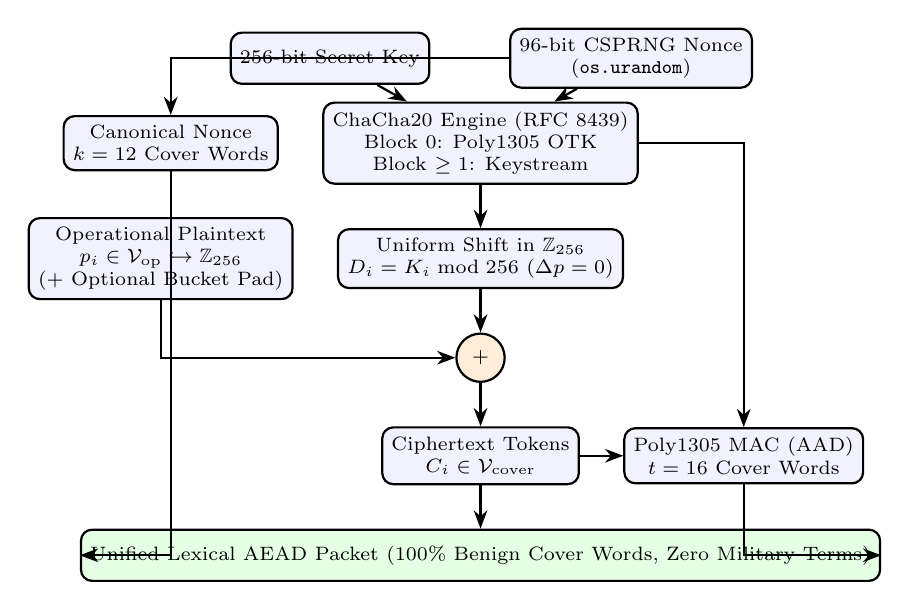
\begin{tikzpicture}[
    node distance=0.85cm and 0.65cm,
    box/.style={rectangle, draw=black, thick, fill=blue!5, rounded corners, minimum height=0.65cm, minimum width=2.2cm, align=center, font=\scriptsize},
    op/.style={circle, draw=black, thick, fill=orange!15, minimum size=0.55cm, align=center, font=\scriptsize\bfseries},
    arr/.style={->, >=Stealth, thick}
]
    \node[box] (key) {256-bit Secret Key};
    \node[box, right=1.0cm of key] (nonce) {96-bit CSPRNG Nonce\\(\texttt{os.urandom})};
    \node[box, below=0.55cm of $(key)!0.5!(nonce)$] (engine) {ChaCha20 Engine (RFC 8439)\\Block 0: Poly1305 OTK\\Block $\ge 1$: Keystream};
    
    \node[box, left=0.55cm of engine] (pre) {Canonical Nonce\\$k=12$ Cover Words};
    \node[box, below=0.55cm of engine] (mod) {Uniform Shift in $\mathbb{Z}_{256}$\\$D_i = K_i \bmod 256$ ($\Delta p=0$)};
    
    \node[box, left=0.55cm of mod] (plain) {Operational Plaintext\\$p_i \in \mathcal{V}_{\text{op}} \hookrightarrow \mathbb{Z}_{256}$\\(+ Optional Bucket Pad)};
    \node[op, below=0.55cm of mod] (add) {$+$};
    \node[box, below=0.55cm of add] (cipher) {Ciphertext Tokens\\$C_i \in \mathcal{V}_{\text{cover}}$};
    \node[box, right=0.55cm of cipher] (poly) {Poly1305 MAC (AAD)\\$t=16$ Cover Words};
    
    \node[box, fill=green!10, below=0.55cm of cipher, minimum width=7.2cm] (pkt) {Unified Lexical AEAD Packet ($100\%$ Benign Cover Words, Zero Military Terms)};

    \draw[arr] (key) -- (engine);
    \draw[arr] (nonce) -- (engine);
    \draw[arr] (nonce) -| (pre);
    \draw[arr] (engine) -- (mod);
    \draw[arr] (plain) |- (add);
    \draw[arr] (mod) -- (add);
    \draw[arr] (add) -- (cipher);
    \draw[arr] (engine) -| (poly);
    \draw[arr] (cipher) -- (poly);
    \draw[arr] (pre) |- (pkt);
    \draw[arr] (cipher) -- (pkt);
    \draw[arr] (poly) |- (pkt);
\end{tikzpicture}%
}
\caption{Decoupled Lexical AEAD architecture ($N=256$ optimal profile): CSPRNG nonce framing, ChaCha20 modular masking over $\mathbb{Z}_{256}$, and RFC 8439 Poly1305 authentication with AAD.}
\label{fig:arch}
\end{figure}

\subsection{Security Analysis: IND-CPA and INT-CTXT Reduction Sketch}
Because our construction modifies RFC 8439 by replacing byte-wise XOR with modular addition over $\mathbb{Z}_N$ and base-$N$ serialization, security must be established explicitly rather than assumed by association:
\begin{itemize}
    \item \textbf{Confidentiality (Nonce-Respecting IND-CPA):} Under the assumption that ChaCha20 is a secure pseudorandom function (PRF) and nonces never repeat under key $K$, the blocks for $b_0 \ge 1$ are computationally indistinguishable from uniform random bytes. When $N=2^b$ ($b \le 16$) or exact rejection sampling is enabled, each displacement $D_i$ is strictly uniform in $\mathbb{Z}_N$ and independent of both $p_i$ and the Poly1305 key (derived from $b_0 = 0$). Because $(\mathbb{Z}_N, +)$ is a finite group, $(\psi(p_i) + D_i) \bmod N$ is a one-time pad over $\mathbb{Z}_N$ for each position $i$, reducing IND-CPA advantage directly to the PRF advantage of ChaCha20.
    \item \textbf{Ciphertext Integrity (INT-CTXT / Non-Malleability):} Suppose an adversary produces a forged packet $\text{Pkt}' = (\text{Pre}', C', \text{Tag}') \neq \text{Pkt}$ or alters $\text{AAD}'$. Canonical range checks enforce strict injectivity on $[0, 2^{96}-1]$ and $[0, 2^{128}-1]$, rejecting any non-canonical or out-of-vocabulary mutation immediately. If $\text{Pre}' \neq \text{Pre}$ represents a distinct valid 96-bit nonce, the derived Poly1305 key $(r', s')$ is fresh and unpredictable under ChaCha20 PRF security. If $\text{Pre}' = \text{Pre}$ and $(\mathcal{C}'_{\text{utf8}}, \text{AAD}') \neq (\mathcal{C}_{\text{utf8}}, \text{AAD})$, forging a valid tag reduces directly to the $\epsilon$-almost-$\Delta$-universal bound of Poly1305 ($\le 8 \lceil |\mathcal{M}|/16 \rceil / 2^{106}$ per forgery attempt \cite{rfc8439}). Because decryption returns plaintext only after constant-time tag verification succeeds, the scheme achieves INT-CTXT and zero wire malleability.
\end{itemize}

\subsection{Asymptotic Complexity and Expansion Dynamics}
For an operational payload of $m$ tokens and cover dimension $N$, the wire token count is $L(m, N) = m + \lceil 96 / \log_2 N \rceil + \lceil 128 / \log_2 N \rceil$, giving expansion ratio $\beta(m, N) = L(m, N) / m$. Table~\ref{tab:expansion} quantifies $\beta(m, N)$ across vocabulary dimensions. At $N=256$, fixed metadata drops to 28 tokens, approaching unity ($\beta = 1.14\times$) at $m=200$.

\begin{table}[htbp]
\caption{Lexical Expansion Ratio $\beta(m, N)$ and Base-$N$ Framing Properties}
\label{tab:expansion}
\centering
\resizebox{\columnwidth}{!}{%
\begin{tabular}{cccccc}
\toprule
\textbf{Size ($N$)} & \textbf{Metadata ($k+t$)} & \textbf{$m = 10$} & \textbf{$m = 50$} & \textbf{$m = 200$} & \textbf{Prop.~1} \\
\midrule
$N = 16$  & $24 + 32 = 56$ tok & $6.60\times$ & $2.12\times$ & $1.28\times$ & Yes \\
$N = 20$  & $23 + 30 = 53$ tok & $6.30\times$ & $2.06\times$ & $1.27\times$ & No \\
$N = 64$  & $16 + 22 = 38$ tok & $4.80\times$ & $1.76\times$ & $1.19\times$ & No \\
$N = 128$ & $14 + 19 = 33$ tok & $4.30\times$ & $1.66\times$ & $1.17\times$ & No \\
$\mathbf{N = 256}$ & $\mathbf{12 + 16 = 28}$ \textbf{tok} & $\mathbf{3.80\times}$ & $\mathbf{1.56\times}$ & $\mathbf{1.14\times}$ & \textbf{Yes} \\
\bottomrule
\end{tabular}%
}
\end{table}

Computationally, generating keystream for $m$ tokens consumes $\lceil m / 64 \rceil$ ChaCha20 blocks for $N \mid 256$ (one byte per token; $\lceil 2m / 64 \rceil$ for the generic 16-bit path) plus $1$ block ($b_0=0$) for the Poly1305 key, totaling $10(1 + \lceil m / 64 \rceil)$ double-rounds ($20(1 + \lceil m / 64 \rceil)$ ARX rounds). Poly1305 executes $\lceil |\mathcal{M}| / 16 \rceil$ modular multiply-accumulate operations in $\mathbb{F}_{2^{130}-5}$. For power-of-two lexicons ($N \in \{16, 256\}$), encryption runs in strictly deterministic $O(m)$ time; under rejection sampling for arbitrary $N$, runtime is expected $O(m)$ (Las Vegas). Our buffered pure-Python reference engine allocates $O(m)$ auxiliary memory for token and MAC buffers, while a streaming C/Rust port can operate in $O(1)$ auxiliary space.

\section{Implementation in Pure Python}
\label{sec:impl}

Minimal containers, forensic triage workstations, and air-gapped hosts often prohibit installing third-party cryptographic wheels or C toolchains. Our reference artifact runs on standard Python 3 using zero external dependencies (relying strictly on standard-library \texttt{os.urandom} for CSPRNG nonces/padding and \texttt{math} for base-$N$ bounds). The artifact comprises four self-contained modules: \texttt{poly1305.py} (RFC 8439 MAC and framing), \texttt{app.py} (ChaCha20 core, generic \texttt{LexicalAEAD} class with $N=256$ benign cover lexicon, canonical bounds, bucket padding, and RFC 8439+Base-256 baseline), \texttt{benchmark.py} (statistical suite with native $t$/$\chi^2$ $p$-values), and \texttt{experimento\_pratico\_dpi.py} (two-regime DPI heuristic simulation).

Listing~\ref{lst:chacha} shows the core ChaCha20 block primitive, canonical range validator, and branchless tag comparison. Bitwise masking with \texttt{0xFFFFFFFF} emulates 32-bit unsigned wrapping, and block counters are explicitly guarded against 32-bit overflow.

\begin{lstlisting}[language=Python, caption={Pure-Python ChaCha20 Core, Canonical Range Check, and Constant-Time Tag Comparison}, label={lst:chacha}]
def rotl32(v: int, c: int) -> int:
    return ((v << c) & 0xFFFFFFFF) | (v >> (32 - c))

def quarter_round(a: int, b: int, c: int, d: int):
    a = (a + b) & 0xFFFFFFFF; d ^= a; d = rotl32(d, 16)
    c = (c + d) & 0xFFFFFFFF; b ^= c; b = rotl32(b, 12)
    a = (a + b) & 0xFFFFFFFF; d ^= a; d = rotl32(d, 8)
    c = (c + d) & 0xFFFFFFFF; b ^= c; b = rotl32(b, 7)
    return a, b, c, d

def _tokens_para_bytes_canonico(self, tokens, nbytes, exp, lbl):
    if len(tokens) != exp:
        raise ValueError(f"{lbl}: expected {exp} tokens.")
    val = 0
    for t in reversed(tokens):
        tok = t.strip().lower()
        if tok not in self.cob_para_id:
            raise ValueError(f"Unknown token '{tok}'.")
        val = val * self.n + self.cob_para_id[tok]
    if val >= (1 << (8 * nbytes)):
        raise ValueError(f"Non-canonical overflow in {lbl}!")
    return [(val >> (8 * i)) & 0xFF for i in range(nbytes)]

def constant_time_compare(a: list[int], b: list[int]) -> bool:
    if len(a) != len(b): return False
    diff = 0
    for x, y in zip(a, b): diff |= (x ^ y)
    return diff == 0
\end{lstlisting}

Automated unit tests in \texttt{app.py} verify 100\% bit-for-bit parity against all 64 output bytes of RFC 8439 Section 2.3.2, the 16-byte Poly1305 vector of Section 2.5.2, and both the full 114-byte ciphertext and 16-byte tag of the Section 2.8.2 AEAD vector. Additional unit proofs confirm zero military keyword leakage under the $N=256$ cover lexicon, 100\% rejection of $+2^{96}$ nonce-overflow, $+2^{128}$ tag-overflow, and out-of-vocabulary injections (always raising uniform \texttt{ValueError} exceptions rather than unhandled \texttt{KeyError}), and exact bucket-padding length equalization. The complete open-source artifact (release \texttt{v1.1.1}, MIT license) is publicly available for independent inspection and reproduction at \url{https://tinyurl.com/2djhbhnn}.

\section{Experimental Methodology and Evaluation}
\label{sec:eval}

All empirical experiments were executed on a single-threaded Apple M1 host (8 cores, 8~GB RAM, macOS 27.2.1) running standard CPython 3.14.7 without external packages, orchestrated via a single reproducibility script (\texttt{executar\_artefacto.sh}) published in the companion repository (\url{https://tinyurl.com/2djhbhnn}, release \texttt{v1.1.1}) that exports raw metrics to JSON files.

\subsection{Strict Avalanche Criterion (SAC)}
The Strict Avalanche Criterion requires that flipping any single input bit inverts each output bit with probability $p = 0.5$ \cite{vaughn2026relaxation, madarrocap2021measuring}. For a 512-bit ChaCha20 block, the theoretical binomial mean is $\mu = 256.00$ bits with standard deviation $\sigma = \sqrt{512 \cdot 0.25} \approx 11.31$ bits. We ran $n = 300$ randomized trials flipping 1 bit in the 256-bit key and $n = 300$ trials flipping 1 bit in the 96-bit nonce, computing exact two-tailed Student's $t$-tests natively inside \texttt{benchmark.py}.

\begin{table}[htbp]
\caption{Strict Avalanche Criterion Dynamics ($n = 300$ Trials, $df = 299$)}
\label{tab:avalanche}
\centering
\resizebox{\columnwidth}{!}{%
\begin{tabular}{lcccc}
\toprule
\textbf{Perturbation Target} & \textbf{Bit Diffusion ($\mu \pm \sigma$)} & \textbf{Ratio} & \textbf{$t$-stat} & \textbf{$p$-value} \\
\midrule
Secret Key (256-bit) & $255.56 \pm 11.50$ & 49.91\% & $-0.668$ & $0.505$ \\
Public Nonce (96-bit) & $255.84 \pm 10.75$ & 49.97\% & $-0.258$ & $0.797$ \\
\midrule
\textit{Binomial Ideal ($H_0$)} & \textit{256.00} $\pm$ \textit{11.31} & \textit{50.00\%} & \textit{0.000} & \textit{---} \\
\bottomrule
\end{tabular}%
}
\end{table}

Table~\ref{tab:avalanche} shows sample means within $0.09\%$ of $256.00$ bits, yielding $p = 0.505$ (key) and $p = 0.797$ (nonce). Failing to reject $H_0: \mu = 256.00$ at $\alpha = 0.05$ confirms empirical behavior consistent with uniform binomial bit diffusion across both key and nonce perturbations.

\subsection{Dispersion and Serial Independence Under Skewed Input}
To stress-test frequency masking, we synthesized a 5,000-token operational stream comprising 85\% \texttt{"atacar"} and 15\% \texttt{"base"} ($N=20$). We compared Static Substitution, modular Vigen\`ere ($L=3$), RC4 Stream Codebook \cite{madarrocap2021measuring}, and our ChaCha20 modular engine with rejection sampling enabled ($\Delta p = 0.00$). We report Shannon entropy $H(X)$, efficiency $\eta = (H / \log_2 20) \times 100\%$, Pearson's $\chi^2$ ($df = 19$) with exact upper-tail $p$-value, and lag-1 serial autocorrelation $r_1$ (95\% white-noise bound $|r_1| < 1.96/\sqrt{5000} \approx 0.0277$).

\begin{table}[htbp]
\caption{Dispersion and Serial Independence on 85\%-Skewed Input ($m=5{,}000, N=20$)}
\label{tab:entropy}
\centering
\resizebox{\columnwidth}{!}{%
\begin{tabular}{lccccc}
\toprule
\textbf{Cipher Scheme} & \textbf{$H$ (bits)} & \textbf{$\eta$ (\%)} & \textbf{$\chi^2$} & \textbf{$p$-value} & \textbf{$r_1$} \\
\midrule
Biased Plaintext Input       & 0.6068 & 14.04\% & 69,668.3 & $<10^{-100}$ & $+0.0162$ \\
Static Substitution Codebook & 0.6068 & 14.04\% & 69,668.3 & $<10^{-100}$ & $+0.0162$ \\
Vigen\`ere Modular ($L=3$)   & 2.1916 & 50.71\% & 19,891.4 & $<10^{-100}$ & $-0.4805$ \\
RC4 Stream Codebook          & 4.3186 & 99.92\% & 23.2     & $0.231$      & $+0.0178$ \\
\textbf{ChaCha20 $\mathbb{Z}_{20}$ (RS)} & \textbf{4.3202} & \textbf{99.96\%} & \textbf{11.8} & $\mathbf{0.895}$ & $\mathbf{+0.0053}$ \\
\midrule
\textit{Expected under $H_0$} & \textit{4.3219} & \textit{100.0\%} & $\mathbb{E}=19.0$ & $\mathcal{U}(0,1)$ & \textit{0.0000} \\
\bottomrule
\end{tabular}%
}
\end{table}

Table~\ref{tab:entropy} confirms that Static Substitution preserves input skewness identically, while Vigen\`ere leaks severe periodic negative autocorrelation ($r_1 = -0.4805$). Note that under a true uniform null hypothesis $H_0$, the expected Pearson statistic is $\mathbb{E}[\chi^2] = df = 19.0$ (not $0.0$). Our ChaCha20 engine achieves $H = 4.3202$ bits ($\eta = 99.96\%$), $\chi^2 = 11.8$ ($p = 0.895$, well within the two-tailed acceptance interval $[8.91, 32.85]$), and $|r_1| = 0.0053 < 0.0277$.

\subsection{NIST SP 800-22 Core Subset and Multi-Lag Autocorrelation}
To complement the SAC and $\chi^2$ evidence with standardized randomness tests, we applied four tests of NIST SP 800-22 Rev.~1a implemented in pure Python (Sections 2.1 to 2.4) to $10^6$ bits formed by the $\mathbb{Z}_{256}$ ciphertext indices of an 85\%-skewed plaintext. All four pass at the NIST significance level $\alpha = 0.01$: Frequency (monobit) $p = 0.2919$, Block Frequency ($M=128$) $p = 0.6080$, Runs $p = 0.4139$, and Longest Run of Ones ($M=10{,}000$) $p = 0.8834$. Extending the lag-1 test of Table~\ref{tab:entropy}, the largest absolute serial autocorrelation over lags $1$ to $10$ of the $N=20$ ChaCha20 output is $\max_k |r_k| = 0.0244$, below the single-test 95\% bound $0.0277$. This is a four-test subset, not the full 15-test suite, and passing it supports statistical quality of the keystream-masked indices but does not constitute a security proof.

\subsection{Vocabulary Scaling and MSB Distinguisher Audit}
Table~\ref{tab:scaling} evaluates lexicon scalability across $N \in \{16, 20, 64, 128, 256\}$ on 5,000 skewed tokens, contrasting naive modular reduction against rejection sampling at $N=20$, alongside an empirical MSB-token audit over 2,000 packets validating Proposition~1.

\begin{table*}[t]
\caption{Vocabulary Scaling ($m=5{,}000$ Skewed Tokens) and MSB-Token Structural Distinguisher Audit ($2{,}000$ Packets)}
\label{tab:scaling}
\centering
\begin{tabular}{lccccc|lccc}
\toprule
\multicolumn{6}{c|}{\textbf{(a) Modular Lexicon Scaling Uniformity}} & \multicolumn{4}{c}{\textbf{(b) Nonce \& Tag MSB-Token Coverage ($2{,}000$ Pkts)}} \\
\textbf{Configuration} & \textbf{$H$} & \textbf{$\log_2 N$} & \textbf{$\chi^2$ ($df$)} & \textbf{$p$-val} & \textbf{Bias $\Delta p$} & \textbf{Field / Profile} & \textbf{Observed} & \textbf{$\chi^2$} & \textbf{$p$-val} \\
\midrule
$N=16$ & 3.9985 & 4.0000 & 10.3 (15) & 0.804 & $0.00$ & $N=20$ Nonce MSB & $2 / 20$ & 18,062.7 & $<10^{-100}$ \\
$N=20$ (Naive mod) & 4.3205 & 4.3219 & 9.6 (19) & 0.962 & $1.53\times 10^{-5}$ & $N=20$ Tag MSB & $7 / 20$ & 4,160.7 & $<10^{-100}$ \\
$N=20$ (Rej. Sampl.) & 4.3202 & 4.3219 & 11.8 (19) & 0.895 & $0.00$ & \textbf{$N=256$ Nonce MSB} & $\mathbf{256 / 256}$ & \textbf{220.3} & \textbf{0.943} \\
$N=64$ & 5.9895 & 6.0000 & 74.2 (63) & 0.158 & $0.00$ & \textbf{$N=256$ Tag MSB} & $\mathbf{256 / 256}$ & \textbf{199.8} & \textbf{0.996} \\
$N=128$ & 6.9827 & 7.0000 & 121.0 (127) & 0.634 & $0.00$ & \multicolumn{4}{l}{\textit{Prop.~1 confirmed: $N=20$ leaks MSB range;}} \\
$\mathbf{N=256}$ \textbf{(Optimal)} & \textbf{7.9649} & \textbf{8.0000} & \textbf{239.8 (255)} & \textbf{0.744} & $\mathbf{0.00}$ & \multicolumn{4}{l}{\textit{$N=256$ attains full uniform coverage ($p > 0.80$).}} \\
\bottomrule
\end{tabular}
\end{table*}

The empirical audit confirms Proposition~1 cleanly. Although rejection sampling eliminates per-token modulo bias at $N=20$ ($\Delta p: 1.53\times 10^{-5} \to 0.00$), base-20 framing still constrains the nonce MSB token to just $2/20$ words ($\chi^2 = 18{,}062.7, p < 10^{-100}$) and the tag MSB token to $7/20$ words ($\chi^2 = 4{,}160.7, p < 10^{-100}$). Moving to $N=256$ eliminates both leaks completely, achieving full $256/256$ coverage with $p = 0.943$ (nonce MSB) and $p = 0.996$ (tag MSB).

\begin{figure}[htbp]
\centering
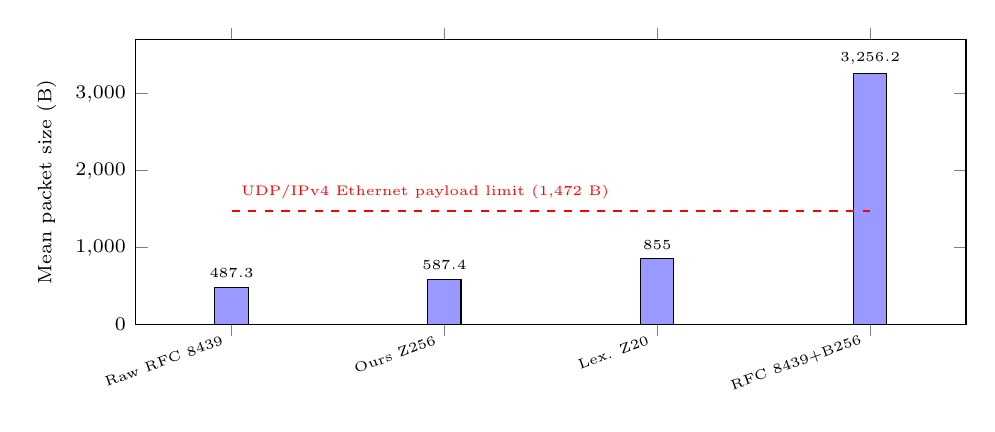
\begin{tikzpicture}
\begin{axis}[
    ybar, width=\columnwidth, height=5.2cm, bar width=12pt,
    symbolic x coords={Raw RFC 8439, Ours Z256, Lex. Z20, RFC 8439+B256},
    xtick=data, x tick label style={font=\tiny, rotate=20, anchor=east},
    ylabel={Mean packet size (B)}, ylabel style={font=\scriptsize},
    ymin=0, ymax=3700, nodes near coords, nodes near coords style={font=\tiny},
    tick label style={font=\scriptsize}, enlarge x limits=0.15]
\addplot[fill=blue!40] coordinates {(Raw RFC 8439,487.3) (Ours Z256,587.4) (Lex. Z20,855.0) (RFC 8439+B256,3256.2)};
\draw[red, thick, dashed] (axis cs:Raw RFC 8439,1472) -- (axis cs:RFC 8439+B256,1472);
\node[red, font=\tiny, anchor=south west] at (axis cs:Raw RFC 8439,1500) {UDP/IPv4 Ethernet payload limit (1,472 B)};
\end{axis}
\end{tikzpicture}
\caption{Mean wire size per 60-word report (1,000 packets/profile) against the Ethernet single-frame limit. The byte-encoded baseline exceeds it by $2.2\times$.}
\label{fig:mtu}
\end{figure}

\begin{figure}[htbp]
\centering
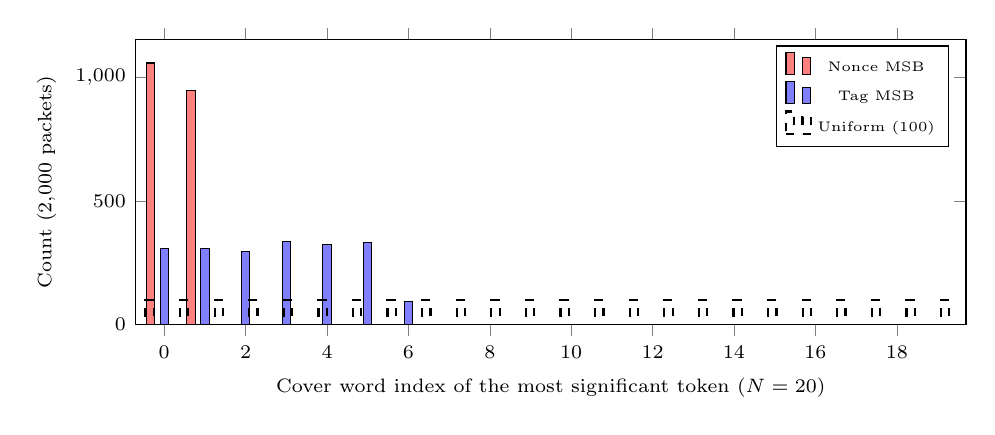
\begin{tikzpicture}
\begin{axis}[
    ybar, width=\columnwidth, height=5.2cm, bar width=3pt,
    xlabel={Cover word index of the most significant token ($N=20$)}, xlabel style={font=\scriptsize},
    ylabel={Count (2,000 packets)}, ylabel style={font=\scriptsize},
    xmin=-0.7, xmax=19.7, ymin=0, ymax=1150, tick label style={font=\scriptsize},
    legend style={font=\tiny, at={(0.98,0.98)}, anchor=north east}]
\addplot[fill=red!50] coordinates {(0,1056) (1,944) (2,0) (3,0) (4,0) (5,0) (6,0) (7,0) (8,0) (9,0) (10,0) (11,0) (12,0) (13,0) (14,0) (15,0) (16,0) (17,0) (18,0) (19,0)};
\addplot[fill=blue!50] coordinates {(0,309) (1,309) (2,295) (3,337) (4,324) (5,333) (6,93) (7,0) (8,0) (9,0) (10,0) (11,0) (12,0) (13,0) (14,0) (15,0) (16,0) (17,0) (18,0) (19,0)};
\addplot[black, dashed, thick, domain=-0.7:19.7] {100};
\legend{Nonce MSB, Tag MSB, Uniform (100)}
\end{axis}
\end{tikzpicture}
\caption{Empirical MSB-token distribution for $N=20$: only 2 (nonce) and 7 (tag) of 20 words ever occur. At $N=256$ all 256 words occur with $p \ge 0.943$ (Table~\ref{tab:scaling}).}
\label{fig:msb}
\end{figure}

\subsection{Multi-Trial Throughput and Baseline Comparison}
To ensure fair benchmarking, we ran warmup iterations followed by $R=30$ timed repetitions per payload scale ($m \in \{50, 500, 2000\}$ operational tokens), reporting mean $\pm$ standard deviation in Table~\ref{tab:throughput}. Beyond raw ChaCha20 modular encryption, we benchmark our complete authenticated \textbf{Lexical AEAD $\mathbb{Z}_{256}$} engine directly against the standard \textbf{RFC 8439 + Base-256 Cover} baseline.

\begin{table*}[t]
\caption{Processing Throughput (Mean $\pm$ Std over $R = 30$ Trials after Warmup) and Unit Latency}
\label{tab:throughput}
\centering
\begin{tabular}{lcccc}
\toprule
\textbf{Cipher / AEAD Scheme} & \textbf{$m = 50$ Tokens} & \textbf{$m = 500$ Tokens} & \textbf{$m = 2{,}000$ Tokens} & \textbf{Unit Cost ($m=2{,}000$)} \\
\midrule
Static Substitution (Unauth.) & $44.2 \pm 3.7$ M/s & $44.3 \pm 0.2$ M/s & $46.9 \pm 0.2$ M/s & $0.02 \pm 0.00$~$\mu$s/tok \\
Vigen\`ere $L=3$ (Unauth.) & $12.0 \pm 0.6$ M/s & $12.0 \pm 0.3$ M/s & $12.0 \pm 0.3$ M/s & $0.08 \pm 0.00$~$\mu$s/tok \\
RC4 Stream Codebook (Unauth.) & $0.98 \pm 0.02$ M/s & $1.95 \pm 0.04$ M/s & $2.17 \pm 0.03$ M/s & $0.46 \pm 0.01$~$\mu$s/tok \\
ChaCha20 Modular Stream ($\mathbb{Z}_{256}$) & $608.6 \pm 21.2$ k/s & $746.3 \pm 13.7$ k/s & $749.9 \pm 35.6$ k/s & $1.34 \pm 0.08$~$\mu$s/tok \\
\midrule
RFC 8439 AEAD + Base-256 Cover & $80.1 \pm 1.1$ k/s & $91.8 \pm 1.0$ k/s & $94.2 \pm 0.8$ k/s & $10.62 \pm 0.09$~$\mu$s/tok \\
\textbf{Lexical AEAD $\mathbb{Z}_{256}$ (Ours, Full AEAD)} & $\mathbf{224.0 \pm 4.2}$ \textbf{k/s} & $\mathbf{415.7 \pm 9.8}$ \textbf{k/s} & $\mathbf{444.9 \pm 10.2}$ \textbf{k/s} & $\mathbf{2.25 \pm 0.05}$~$\boldsymbol{\mu}\mathbf{s/tok}$ \\
\bottomrule
\end{tabular}
\end{table*}

Two findings stand out. First, adding full Poly1305 authentication, AAD framing, and canonical nonce/tag serialization reduces ChaCha20 pure-Python throughput from $749.9$~k to $444.9$~k tokens/s ($2.25$~$\mu$s/token), well under 1~ms for typical 50-to-200-word operational messages. Second, our ring-based Lexical AEAD outperforms standard RFC 8439 + Base-256 Cover by $\mathbf{4.72\times}$ at $m=2{,}000$ ($444.9$~k vs. $94.2$~k tokens/s), because encrypting indexed semantic tokens consumes only 1 keystream byte per operational word rather than encrypting every UTF-8 character byte ($\sim 7.5$~bytes/word) and authenticating a much larger ciphertext body.

\subsection{Two-Regime Simulated Heuristic DPI and Anti-Tamper Evaluation}
To evaluate perimeter concealment honestly without conflating stateless heuristics with commercial appliances or ML flow classifiers, we implemented a controlled \textbf{simulated stateless DPI testbed} (\texttt{experimento\_pratico\_dpi.py}) evaluating three canonical middlebox rules across 10,000 packets (1,000 packets per profile across two payload regimes):
\begin{enumerate}
    \item \textbf{F1 (Byte-Entropy Filter):} Flags payloads with $H_b \ge 6.8$ bits/byte.
    \item \textbf{F2 (Non-Printable Ratio Filter):} Flags payloads with printable ASCII density $\rho_{\text{print}} < 85\%$.
    \item \textbf{F3 (Operational Keyword Watchlist IDS):} Flags plaintext or lexical payloads containing sensitive tactical terms (\texttt{atacar}, \texttt{evacuar}, \texttt{reforcos}, \texttt{combustivel}, \texttt{recuar}, \texttt{urgente}).
\end{enumerate}

Crucially, we evaluate both \textbf{Regime A (Short Tactical Commands, 6 words / $\sim 45$~B)} and \textbf{Regime B (Extended Operational Reports, 60 words / $\sim 459$~B)}. In short binary frames ($\sim 73$~B), byte entropy is mathematically bounded by $\log_2(73) \approx 6.19 < 6.8$, meaning F1 never triggers on short raw binary frames; evaluating Regime B exposes the full behavior of both F1 and F2 simultaneously.

\begin{table*}[t]
\caption{Simulated Stateless Heuristic DPI Evaluation Across Two Payload Regimes ($1{,}000$ Packets/Profile per Regime)}
\label{tab:dpi_eval}
\centering
\begin{tabular}{llccccccccc}
\toprule
\textbf{Regime} & \textbf{Traffic Profile} & \textbf{Mean $H_b$} & \textbf{Print.} & \textbf{Size (B)} & \textbf{Tok.} & \textbf{F1:Ent} & \textbf{F2:Bin} & \textbf{F3:IDS} & \textbf{Evade} & \textbf{Lat. ($\mu$s)} \\
\midrule
\multirow{5}{*}{\shortstack[l]{\textbf{Regime A}\\Short Cmds\\(6 words)}}
& Plaintext Tactical & 3.6291 & 100.0\% & 45.0 & 6 & 0.0\% & 0.0\% & 100.0\% & 0.0\% & 0.1 \\
& Raw RFC 8439 Binary & 5.9189 & 38.7\% & 73.0 & --- & 0.0\% & 100.0\% & 0.0\% & 0.0\% & 175.1 \\
& Lexical AEAD $\mathbb{Z}_{20}$ (Legacy) & 3.8608 & 100.0\% & 443.0 & 59 & 0.0\% & 0.0\% & 100.0\% & 0.0\% & 185.8 \\
& RFC 8439 + Base-256 Cover & 3.8586 & 100.0\% & 486.4 & 73 & 0.0\% & 0.0\% & 0.0\% & 100.0\% & 179.2 \\
& \textbf{Lexical AEAD $\mathbb{Z}_{256}$ (Ours)} & \textbf{3.8282} & \textbf{100.0\%} & \textbf{226.4} & \textbf{34} & \textbf{0.0\%} & \textbf{0.0\%} & \textbf{0.0\%} & \textbf{100.0\%} & \textbf{181.5} \\
\midrule
\multirow{5}{*}{\shortstack[l]{\textbf{Regime B}\\Ext. Reports\\(60 words)}}
& Plaintext Tactical & 3.8646 & 100.0\% & 459.3 & 60 & 0.0\% & 0.0\% & 100.0\% & 0.0\% & 0.2 \\
& Raw RFC 8439 Binary & 7.5673 & 38.3\% & 487.3 & --- & 100.0\% & 100.0\% & 0.0\% & 0.0\% & 774.7 \\
& Lexical AEAD $\mathbb{Z}_{20}$ (Legacy) & 3.8789 & 100.0\% & 855.0 & 113 & 0.0\% & 0.0\% & 100.0\% & 0.0\% & 331.5 \\
& RFC 8439 + Base-256 Cover & 3.8853 & 100.0\% & 3,256.2 & 487 & 0.0\% & 0.0\% & 0.0\% & 100.0\% & 786.5 \\
& \textbf{Lexical AEAD $\mathbb{Z}_{256}$ (Ours)} & \textbf{3.8660} & \textbf{100.0\%} & \textbf{587.4} & \textbf{88} & \textbf{0.0\%} & \textbf{0.0\%} & \textbf{0.0\%} & \textbf{100.0\%} & \textbf{237.9} \\
\bottomrule
\end{tabular}
\end{table*}

Table~\ref{tab:dpi_eval} reveals three decisive operational insights:
\begin{enumerate}
    \item \textbf{Decomposition of Binary Detection:} On short commands (Regime A), Raw RFC 8439 Binary is caught exclusively by F2 (printability, 100.0\%) while F1 stays at 0.0\% ($H_b = 5.9189$). On extended reports (Regime B), binary payloads reach $H_b = 7.5673$, triggering \emph{both} F1 (100.0\%) and F2 (100.0\%).
    \item \textbf{Necessity of Lexicon Decoupling:} Both Plaintext Tactical and legacy $\mathbb{Z}_{20}$ Lexical AEAD emit tactical words on the wire and fail F3 (100.0\% watchlist alerts). Decoupling to our benign 256-word cover lexicon reduces F3 alerts to 0.0\%.
    \item \textbf{Wire Efficiency vs. Standard Byte-Word Encoding:} Although RFC 8439 + Base-256 Cover also achieves 100\% evasion across F1--F3, it bloats 60-word reports to $3,256.2$~B (487 tokens), exceeding the 1,500-byte Ethernet MTU by more than $2\times$ and forcing IP fragmentation. Our $\mathbb{Z}_{256}$ Lexical AEAD transmits the exact same report in $587.4$~B (88 tokens) at $237.9$~$\mu$s, achieving an \textbf{82.0\% wire-size reduction} and \textbf{$3.31\times$ lower latency} while remaining comfortably inside a single Ethernet frame (only $1.21\times$ the raw binary payload size).
\end{enumerate}

\subsection{Red-Team Self-Attack: Zipf Likelihood-Ratio Detector and UDP Loopback}
\label{sec:redteam}
To quantify the limit stated in our threat model rather than only assert it, we implemented an adversary that knows the cover lexicon and applies a likelihood-ratio test between a Zipf ($s=1$) prose model and the uniform model over the 256 cover words. Natural traffic is a synthetic Zipf proxy, not a real corpus, so the figures bound a best case for the attacker under that assumption. Over 1,000 trials per window, the detector flags our $\mathbb{Z}_{256}$ stream in $99.2\%$ of windows of $W=10$ tokens, $99.9\%$ at $W=20$, and $100.0\%$ at $W=40$ and $W=88$, while accepting Zipf prose in $98.3\%$, $100\%$, $100\%$, and $100\%$ of windows respectively. The scheme therefore does \emph{not} resist a linguistic-statistics adversary; its stealth claim is restricted to stateless entropy, printability and keyword filters.

We also transmitted 300 datagrams per profile of 60-word reports through a real UDP socket on the loopback interface (Python \texttt{socket}) and applied F1 to F3 to the received datagrams: all 300 raw binary datagrams were flagged, none of the Base-256 or Lexical AEAD datagrams were flagged, and all 300 Base-256 datagrams exceeded the 1,472-byte Ethernet payload limit while none of ours did. This is a transport-realistic but still single-host test; reference Snort/Suricata rules for F2 and F3 are published in the artifact repository (\texttt{ids\_rules/}) but were not executed on a live sensor in this paper.

Finally, across 1,000 controlled adversarial tampering trials evenly split into four attack classes (250 ciphertext mutations, 250 nonce preamble mutations, 250 Poly1305 tag mutations, and 250 AAD modifications, out-of-vocabulary injections, and $+2^{96}$ non-canonical overflow forgeries), decryption rejected \textbf{1,000 / 1,000 (100.0\%)} forged frames with zero false acceptances.

\section{Operational Constraints and Threat Modeling}
\label{sec:constraints}

\subsection{Two-Time Pad Hazard and Nonce Management}
Stream ciphers lose confidentiality if a key-nonce pair is ever reused \cite{rfc8439}. Encrypting two messages $P^{(1)}$ and $P^{(2)}$ under identical $(K, N_{\text{pub}})$ cancels displacements $D_i$:
\begin{equation}
\phi(C_i^{(1)}) - \phi(C_i^{(2)}) \equiv \psi(P_i^{(1)}) - \psi(P_i^{(2)}) \pmod N
\end{equation}
and exposes the Poly1305 one-time key $(r, s)$ to polynomial root-finding forgery. Our implementation defaults to generating a fresh 96-bit nonce per message via the operating system CSPRNG (\texttt{os.urandom(12)}) serialized as an in-band preamble. Under random 96-bit nonces, the birthday collision bound limits safe single-key volume to roughly $2^{32}$ messages (collision probability $\le 2^{-33}$); stateless high-volume deployments should rekey periodically or adopt 192-bit XChaCha20 nonces.

\subsection{Modulo Truncation Bias and Rejection Sampling}
Naive modular reduction $K_i \bmod N$ incurs bias $\Delta p = 1 / 65{,}536 \approx 1.526 \times 10^{-5}$ whenever $N \nmid 2^{16}$ (e.g., $N=20$). Enabling rejection sampling by default for non-power-of-two lexicons forces $\Delta p = 0.00$ with negligible rejection rate $p_{\text{reject}} = (65{,}536 \bmod N) / 65{,}536 < 0.031\%$ ($\forall N \le 256$). Note that rejection sampling introduces a minor keystream-dependent execution branch; adopting our Proposition~1 optimal profile ($N=256$) avoids rejection sampling altogether, achieving $\Delta p = 0.00$ with strictly branchless keystream extraction.

\subsection{Constant-Time Verification and CPython Microarchitectural Limits}
Early-exit equality checks on MAC tags enable remote byte-by-byte forgery via timing side channels. Our pure-Python \texttt{constant\_time\_compare} accumulates bitwise XOR differences across all 16 tag bytes without short-circuit returns. In production Python deployments where standard-library C helpers are acceptable, \texttt{hmac.compare\_digest} should be preferred over interpreted loops because CPython introduces secondary microarchitectural jitter from boxed integer allocation, dynamic heap objects, and garbage collection \cite{aamir2021chacha20}. Environments with local co-resident timing adversaries require compiled C or Rust implementations.

\subsection{Length Fingerprinting and Authenticated Bucket Padding}
Because unpadded lexical encryption preserves a 1:1 token count ($m = |\text{Pkt}| - 28$ at $N=256$), packet length leaks plaintext word count. To mitigate volumetric traffic analysis, \texttt{app.py} implements authenticated randomized bucket padding (\texttt{pad\_bucket}): prior to encryption, a 2-token base-$N$ length header and CSPRNG-sampled cover tokens pad the plaintext to a fixed bucket size (e.g., $\mathcal{B} \in \{64, 128, 256\}$). Unit Test~5 confirms that 2-word and 8-word messages pad to identical 92-token frames under $\mathcal{B}=64$ while remaining fully authenticated by Poly1305.

\subsection{Threat Model Boundaries: Stateless DPI vs. Linguistic and Flow Classifiers}
Clear adversarial boundaries are essential for honest evaluation:
\begin{enumerate}
    \item \textbf{In-Scope (Stateless Perimeter DPI and Watchlist Filters):} Middleboxes enforcing byte-entropy thresholds ($H_b \ge 6.8$), ASCII printability limits ($\rho_{\text{print}} < 85\%$), binary tunnel headers, and operational keyword signatures. Against this threat model, our decoupled $\mathbb{Z}_{256}$ Lexical AEAD achieves 100\% evasion ($H_b = 3.8660$, $\rho_{\text{print}} = 100\%$, zero watchlist hits) within single-MTU frames.
    \item \textbf{Out-of-Scope (Linguistic $n$-Gram, Zipf, and Deep Flow Classifiers):} Because output cover words follow a uniform distribution over $\mathcal{V}_{\text{cover}}$, sequences violate Zipf's Law and natural grammatical transitions ($P(w_i \mid w_{i-1}) \approx 1/256$). Specialized statistical $n$-gram anomaly detectors or neural language classifiers \cite{adeeb2025steggpt, wang2025multiclassification} can distinguish uniform word lists from natural prose, and timing/inter-arrival classifiers \cite{sun2022deep, alazzam2026advanced} operate independently of payload content. Defeating linguistic steganalysis requires grammar-constrained encoding, discussed next.
\end{enumerate}

\section{Future Research Directions}
\label{sec:future}

Three concrete engineering extensions follow directly from our threat-model boundaries:

\textbf{Syntax-Constrained Cover Encoders via CFGs:} Mapping uniform $\mathbb{Z}_{256}$ residues into slot-constrained Context-Free Grammars or Part-of-Speech templates (where each syntactic slot draws from a $2^b$-sized word class) would preserve zero-bias security while matching natural syntactic structure and resisting $n$-gram detectors without LLM inference overhead.

\textbf{Live Network Appliance and ML Classifier Benchmarks:} Deploying the protocol over real UDP/HTTP covert transports and measuring detection rates against live Suricata/Zeek rulesets and trained flow-level classifiers will extend our stateless heuristic evaluation to full-stack network telemetry.

\textbf{Embedded C and MicroPython Ports:} Porting the $N=256$ Lexical AEAD core to constant-time C and MicroPython on constrained microcontrollers (ESP32, RP2040) will enable profiling of power draw, RAM usage, and side-channel emissions on low-bandwidth LoRa and VHF/UHF links.

\section{Conclusion}
\label{sec:conclusion}

This paper presented the design, formal framing analysis, pure-Python implementation, and empirical evaluation of a dependency-free Lexical AEAD engine built on RFC 8439 ChaCha20-Poly1305. By decoupling operational commands from a 256-word benign cover lexicon, enforcing canonical base-$N$ range validation, generating CSPRNG nonces, supporting AAD and authenticated randomized bucket padding, and proving the Base-$N$ Divisibility Proposition, the architecture resolves classical codebook vulnerabilities while eliminating both non-canonical malleability and MSB-token distinguishers present in non-power-of-two designs ($N=20$). The implementation passes 100\% of bytes in official RFC 8439 Sections 2.3.2, 2.5.2, and 2.8.2 test vectors, satisfies SAC targets ($49.91\%$ key and $49.97\%$ nonce diffusion), eliminates frequency bias under 85\%-skewed inputs ($H = 4.3202$, $\chi^2 = 11.8$, $p = 0.895$), and sustains $444.9$~k authenticated tokens/s in pure Python. Across 10,000 simulated stateless DPI packets spanning short and extended payloads, the decoupled $\mathbb{Z}_{256}$ scheme achieves 100\% evasion across byte-entropy, printability, and keyword-watchlist rules while cutting wire size by 82.0\% and accelerating throughput by $4.7\times$ over standard RFC 8439 + Base-256 encoding, with 100.0\% rejection across 1,000 four-vector tampering trials.

\bibliographystyle{IEEEtran}
\bibliography{referencias}

\end{document}
